\section{Sample section}
\label{sec1}

Sample text. Sample text. Sample text. Sample text. Sample text. Sample text. 
Sample text. Sample text. Sample text. Sample text. Sample text. Sample text. 
Sample text. Sample text. Citation of Einstein paper~ \\\citet{01_B_LagrMech}. \\
\begin{figure}[h]
    \centering
    \begin{subfigure}[t]{0.5\textwidth}
        \centering
        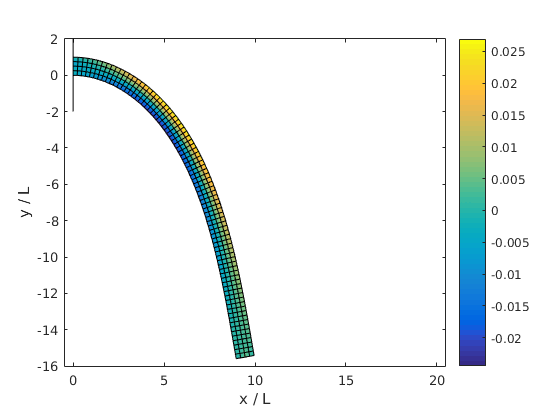
\includegraphics[width=5cm]{data/a}
        \caption{}\label{a}
    \end{subfigure}%
    ~ 
    \begin{subfigure}[t]{0.5\textwidth}
        \centering
        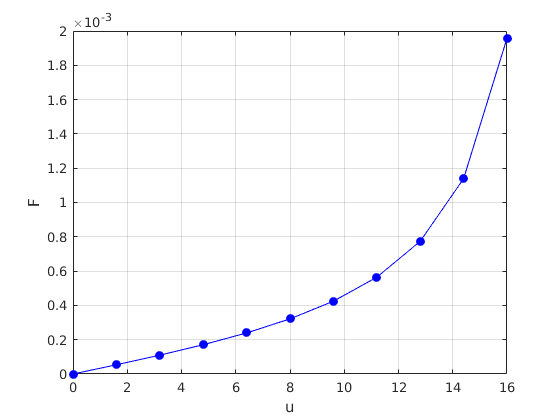
\includegraphics[width=5cm]{data/b}
        \caption{}\label{b}
    \end{subfigure}
    \caption{Caption place holder \subrefnew{a} \subrefnew{b}} \label{fig}
\end{figure}
\\
\figref{fig}\subrefnew{a}
\\
\citet{01_SotA_cohes_dyn} \\
\citet{02_SotA_cohes} \\
\citet{03_SotA_virtClos} \\
\citet{01_PF_dyn_brittle} \\
\citet{02_PF_HO_brittle} \\
\citet{03_PF_ductile} \\
\citet{04_PF_HO_finDef} \\
\citet{05_PF_ductile} \\
\citet{06_PF_ductile}

\begin{align}
\begin{aligned}   \label{1}
1=1 \\
2=2 
\end{aligned}
\end{align}
bla ${\eqref{1}}_{1}$

\subsection{Sample subsection} \label{subsec1}

Sample text. Sample text. Sample text. Sample text. Sample text. Sample text. 
Sample text. Sample text. Sample text. Sample text. Sample text. Sample text. 
Sample text. 